\documentclass{article}
\usepackage{amsthm}
\usepackage{amsmath}
\usepackage{graphicx}
\usepackage{subfigure}
\usepackage{verbatim}
\usepackage{glossaries}
\usepackage{epstopdf}
\newtheorem{theorem}{Theorem}[section]
\newtheorem{corollary}[theorem]{Corollary}
\newtheorem{defination}{Definition}[section]
\newtheorem{proposition}{Proposition}[section]
\begin{document}
\section{Approach}
In this article, we name the MAC scheme adopted in Cost-Effective Tag Design\cite{} CETD-MAC. 
\subsection{Background of CETD-MAC and Security Definitions}
\paragraph{Notations of Symbols}
Let \{0,1\}$^n$ be the set of all n-bit binary strings. The set of all binary string is expressed as \{0,1\}$^*$.  
For a string X $\in$ \{0,1\}$^n$, |X| is its length in bits, and $\vert$ X $\vert$ $_l$ = $\lceil$$\vert$ X $\vert$/l$\rceil$ is the length of X in l-bit blocks.  Let 0$^l$ and 1$^l$ denote bit strings of all zeros and all ones. 
For a bit string X and an integer l that $\vert$ X $\vert$ $\geq$ l, msb$_l$(X) denotes the most significant l bits(left most l bits) of X and lsb$_l$(X) for least significant l bits(right most l bits) of X.
For two bit string X and Y, we denote X$\|$Y  or XY as the their concatenation. For bit string X whose length in bits is multiple of integer l, we denote X parted into l-bit sub-strings as X = (X[1]X[2]$\ldots$X[n])$_l$, where X[1], X[2], $\ldots$, X[n] $\in$ \{0,1\}$^l$.
The number of bits in a string of X is denoted as len(X).

The block cipher encryption of a string X with a secret key K is denoted as E$_K$(X). E$_K$(X) expresses the String mapping of \{0,1\}$^n$ $\rightarrow$ \{0,1\}$^n$ where n is the len(X) and len(output).

\paragraph{Specification of Cost-Effective Tag Design and CETD-MAC}
In this section, we depict the design details of CETD-MAC scheme. At the beginning we express notations required to understand CETD-MAC scheme. 
\paragraph{Definition of CETD-MAC Scheme}
CETD-MAC scheme can be expressed as tag = CETD-MAC(M, nonce-input). The input arguments of CETD-MAC are message M and a tuple named nonce-input. The tuple nonce-input is the concatenation of the memory address of M, a counter and a random number, denoted as nonce-input=(address$\|$counter$\|$random). The length of nonce-input, len(nonce-input), is identical to the length of input to block cipher E$_K$(X). The output of CETD-MAC is named tag, whose length is optional. We use Sub-BLK-No to express the value of len(M)/len(tag). One preliminary of CETD-MAC is that Sub-BLK-No should be no less than 2 to assure that swapping stage can work and 0s will be concatenated to the leftmost of input message when Sub-BLK-No is not integer.  
The concept of CETD-MAC is expressed in Figure $\ref{CETD-MAC}$.
\begin{figure}[htbp]
 \centering
 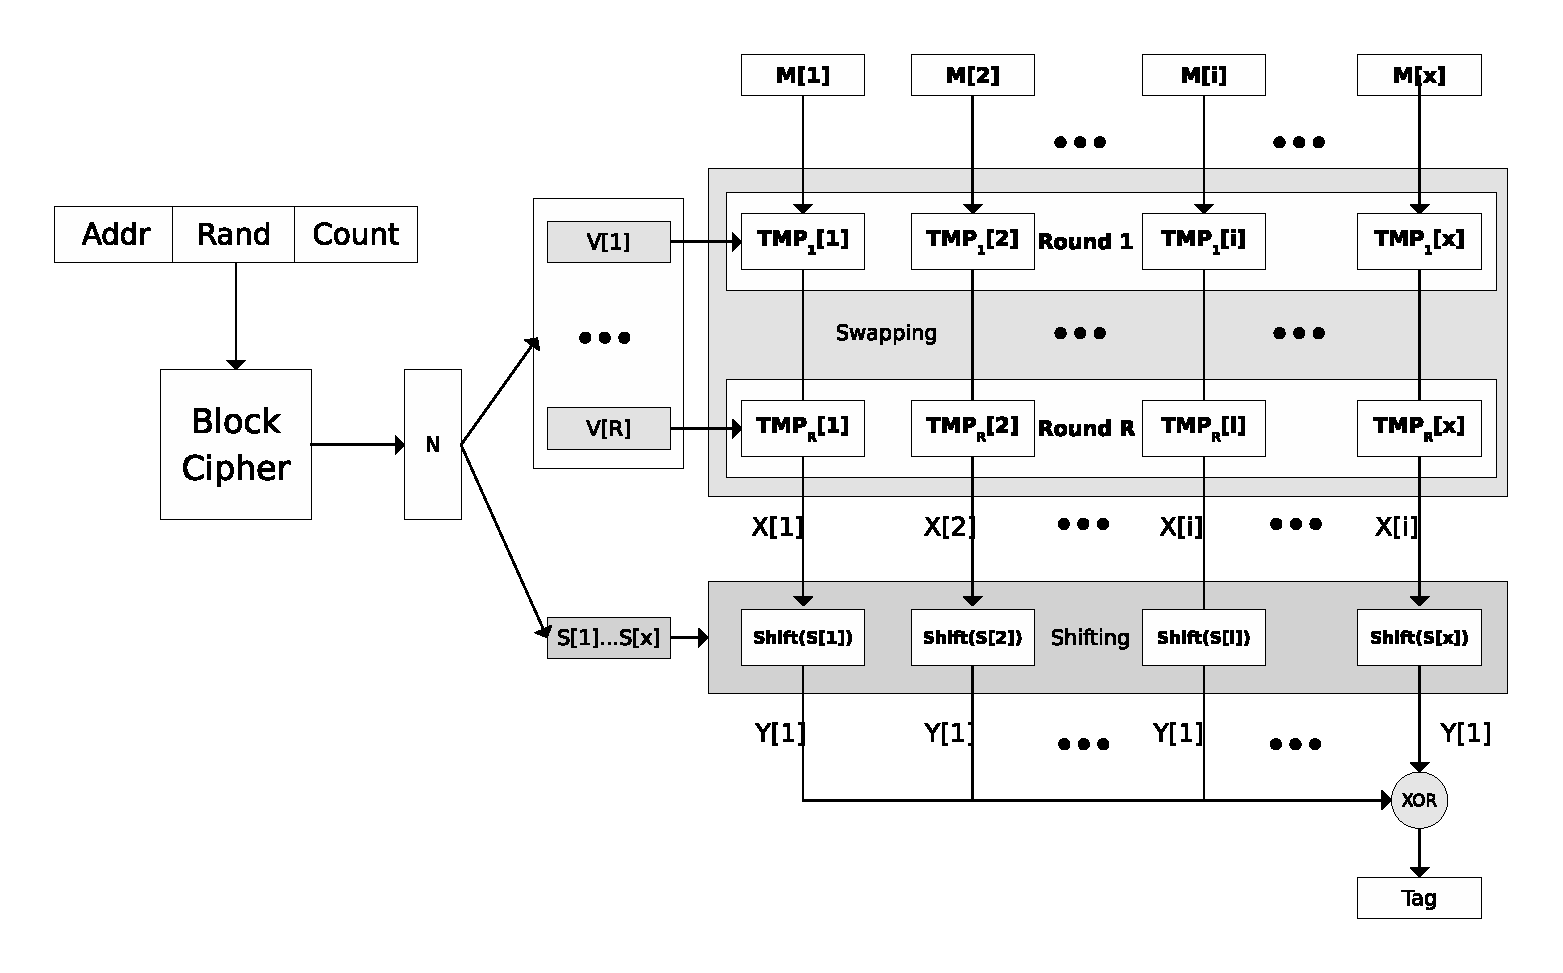
\includegraphics[scale=0.6]{./diagrams/CETD.eps}
 \caption{The CETD-MAC Scheme}
 \label{fig:CETD-MAC}
\end{figure}

\begin{figure}[htbp]
 \centering
 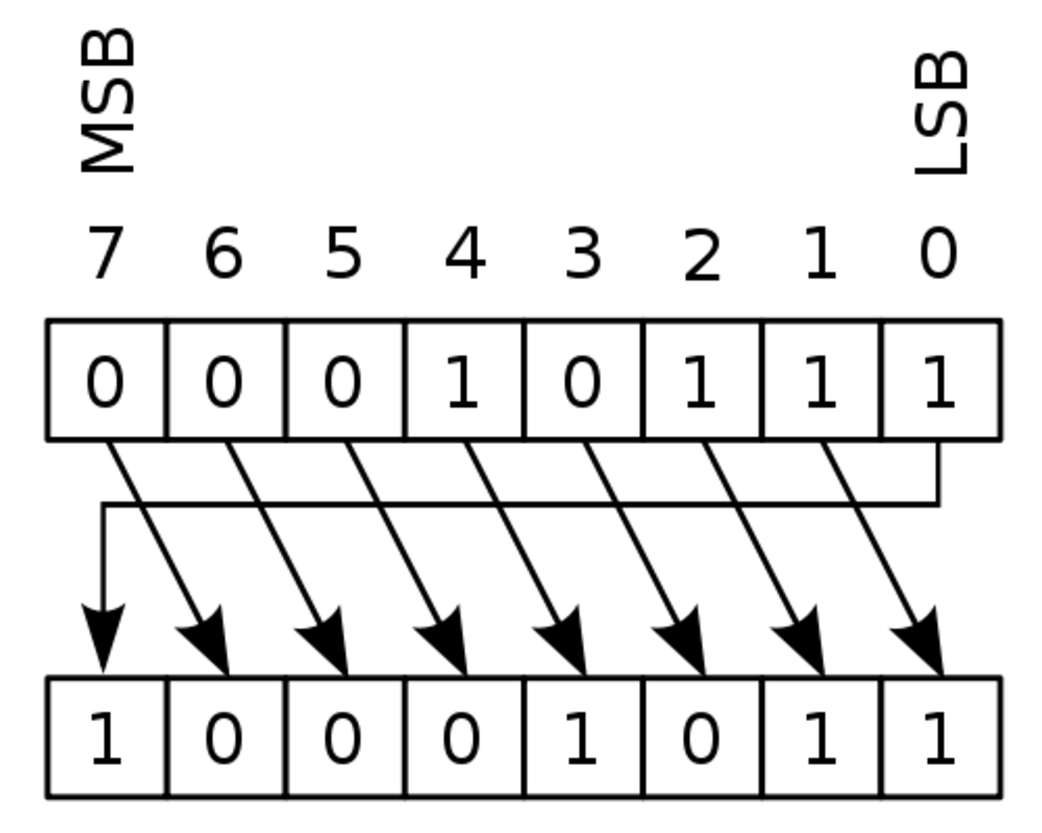
\includegraphics[scale=0.4]{./diagrams/rotate_right.pdf}
 \caption{The Concept of Rotate Shifting(Right)}
 \label{fig:rotate_shift}
\end{figure}
We follow the definition of CETD-MAC in \cite{keylist}. 
\begin{itemize}
	\item Message is splitted to sub-blocks each of whose length is tag length
	\item The first stage is several rounds of bit-segment swapping. For each round , two sub-blocks are randomly chosen. Introduce shuffle parameter V[i]
	\item The output sub-blocks from swapping stage, named X blocks, are sent to block-level rotate shifting stage. Each X block is rotate shifted for several bits. The concept of rotate shifting is expressed in Fig $\ref{fig:rotate_shift}$ Introduce shift parameter S[i]
	\item The output sub-blocks from shifting stage, named Y blocks, are XORed to form the final tag
\end{itemize}
As the nonce is generated by block cipher encryption E$_K$. Assume E$_K$ performance like a ideal random value generator, for two distinct input nonce-input1 and nonce-input2, the corresponding nonce values N1 and N2 should be random and the probability that N1 is identical to N2 should be 1/2$^n$, where n is len(N1). 

\paragraph{Security Definitions of MAC Schemes under Replay Attacks}
Our security definition of MAC schemes under replay attack follows the definition chosen-message attack. 
An adversary is given access to a tag generation black-box(named oracle) and a message-tag pair verification oracle. The encryption key is maintained unchanged while the nonce value is updated for each calling of tag generation oracle no matter whether the value of input message collide with a value in old timestamp. Secret key and nonces are kept in trusted area and cannot be acquired by the adversary. The adversary can copy the message-tag pairs in old time stamp. When conducting the replay attack, the adversary replaces a memory frame containing a data-tag pair in new timestamp with a copy from his storage. The forgery advantage F$_{CETD-MAC}$ under replay attack is the probability that the adversary can get the verification oracle to accept the replace data-tag pair.  

Assume the copy with old timestamp from the adversary is expressed as (M,T1) where M is the message and T1 is the corresponding tag, and the nonce of (M,T1) is denoted as N1. When applying M to the tag generation at a new time point, we mark the corresponding tag T2 and the nonce N2. If the adversary can succeed a replay attack, then T1 is identical to T2 regardless of the equality of N1 and N2.
Then F$_{CETD-MAC}$ under replay attack can be denoted as the probability Pr[T1 = T2 $\mid$ Message value is M \& N1,N2 are randomly generated]. 

According to the design of CETD-MAC, the tag can be expressed as Y[1]$\oplus$Y[2]$\oplus$$\ldots$$\oplus$Y[x], x is the number of input sub-blocks to CETD-MAC. If the following equation is met:
Y$_1$[1]$\oplus$Y$_1$[2]$\ldots$$\oplus$Y$_1$[x]$\oplus$Y$_2$[1]$\oplus$Y$_2$[2]$\ldots$$\oplus$Y$_2$[x] = 0, where Y$_1$ blocks produce T1 and Y$_2$ blocks generate T2, then T1 is identical to T2. This equation indicates that the behaviour of block-level rotate shifting stage effect the probability of tag collision directly. For easy understanding, we firstly analyze the case that shuffle stage does not work under replay attack, which means X$_1$[i] is identical to X$_2$[i] for any i$\in$[1,x]. The analysis of effect from shuffle stage on X blocks follows then.
\paragraph{The Security of Cost-Effective Tag Design under Replay Attack}
In replay attack, the adversary replace the memory frame written in new time
point Time$_2$ with a copy from old time stamp Time$_1$. The content in memory
frame is a data-tag pair. To defend the replay attack, a tuple(address, counter,
random number) is adopted as input to block cipher encryption to generate the
nonce, which serves the control parameter for each stage in tag generation. The
tuple is distinct for each data message. Assume the block cipher adopted behaves
like PRF, the nonce under replay attack is random and distributed
uniformly for each data message. To Cost-Effective Tag design, the security of integrity of data message replys on the
security of CETD-MAC scheme.

\subsection{Security Weakness of CETD-MAC under Replay Attack}
 We denote the data M and the tag in the forgery frame T1. The output blocks from shuffle stage in generating T1 is denoted as X1 blocks and the output from shifting stage are Y1 blocks. When the forgery frame is read to be verified, the output or shuffle stage is X2 blocks and Y2 blocks for the output from shifting stage. The tag generated by verification is T2.  
As depicted in above section, if the MAC scheme is secure under replay attack,
the tags should be random and distributed uniformly with repeated inputs. This
property ensure the probability the replayed data-tag pair passing verification
is low. If the tags from a MAC scheme have high probability to be identical for
repeated inputs, the MAC scheme is vulnurable to replay attack.

In this section, we depict the weaknesses we found in CETD-MAC under replay attack. These weaknesses let the CETD-MAC to produce tags with high collision probability with some chosen inputs. The tags with highly collision probability ease the adversary`s attack. 
\paragraph{Exposing the Weakness of CETD-MAC}
As the security of CETD-MAC is not provided in \cite{}, we do not know the randomness of tags under replay attack. To begin with, we conduct a simulation of replay attack on two-block 16-bit inputs in the range from 0x0000 to 0xFFFF. Figure $\ref{}$ expresses the tag distinction rate(TDR) which is the value of dividing the number of distinct tag values with the size of tag value domain. We can see that for some specific inputs the TDR is extramely low which means the collision probability is high. The experiment results expressed in Figure $\ref{}$ introduce the motivation of systematically analyzing the security of CETD-MAC under replay attack. We examined the behaviour of each stage in CETD-MAC scheme and found that each stage have a set of inputs with high probability leading output collision.

\subsubsection{Weakness of Shuffle Stage}
Table $\ref{}$ expresses the binary format of the input value resulting low tag distinction rate(below 0.1). We can see that in the two blocks of any input in the table, there is at most one bit whose value is distinct with others. According to the design of shuffle stage, in each round two blocks will do bit segment swapping to exchange bits. For input message like the instances in Table $\ref{}$, the bit distribution cannot be effectly changed, which means ther is high probability that the output of shuffle stage is identical to or has the same blocks as the input message of CETD-MAC. 

\subsubsection{Weakness of Shifting Stage}
\paragraph{XOR Operation and Tag Collision}
The tag T from CETD-MAC can be expressed as the following Equation $\ref{tag_expression}$:
\begin{equation}
	$$T = Y[1]$\oplus$Y[2]$\oplus$$\ldots$$\oplus$Y[x]$$	
\label{tag_expression}
\end{equation}
Then Pr[T1 = T2] can be expressed as the Equation $\ref{tag_collision_exp}$: 
\begin{equation}
	$$Pr[T1 = T2] =
Y$_1$[1]$\oplus$Y$_1$[2]$\oplus$$\ldots$$\oplus$Y$_1$[x]$\oplus$Y$_2$[1]$\oplus$Y$_2$[2]$\oplus$$\ldots$$\oplus$Y$_2$[x]$$	
\label{tag_expression}
\end{equation}
We define the concept "equivalent set" as the set whose elements are identical.
We denote Y$_{all}$ as Y1$\cup$Y2, and Y$_{sub}$ as a sub-set of Y$_{all}$.
$\sum_{i=1}^x$$\oplus$ Y$_{sub}$[i] is denoted as
Y$_{sub}$[1]$\oplus$$\ldots$$\oplus$Y$_{sub}$[x]. Assume Y$_{sub}$ is an
equivalent set, then $\sum_{i=1}^x$$\oplus$ Y$_{sub}$[i] is identical to 0 if x
is an even number and to Y$_{sub}$[1] if x is an odd number.

Assume Y$_{all}$ can be splitted to several distinct equivalent Y$_{sub}$ sets
and the number of distinct Y$_{sub}$ sets each of whom contains odd number of elements is k, then the
result of $\sum_{i=1}^2x$$\oplus$ Y$_{all}$[i] can be expressed as
$\sum_{i=1}^k$$\oplus$ Y$_{dist}$[i], where Y$_{dist}$ is denoted as the set of
k distinct values. The Pr[T1 = T2] is identical to $\sum_{i=1}^k$$\oplus$
Y$_{dist}$[i]. 

We can see that the probability of tag collision is determined by the number of
distinct values in the union of Y1 and Y2, which are the output sets from rotate
shifting stage. If the shifting stage can not ensure the randomness of Y sets
for some repeated X sets, the related tags have high probability to collide.
\begin{figure}
\centering
\subfigure[Same Block Shifted Different Bits]{
\begin{minipage}[b]{0.45\textwidth}
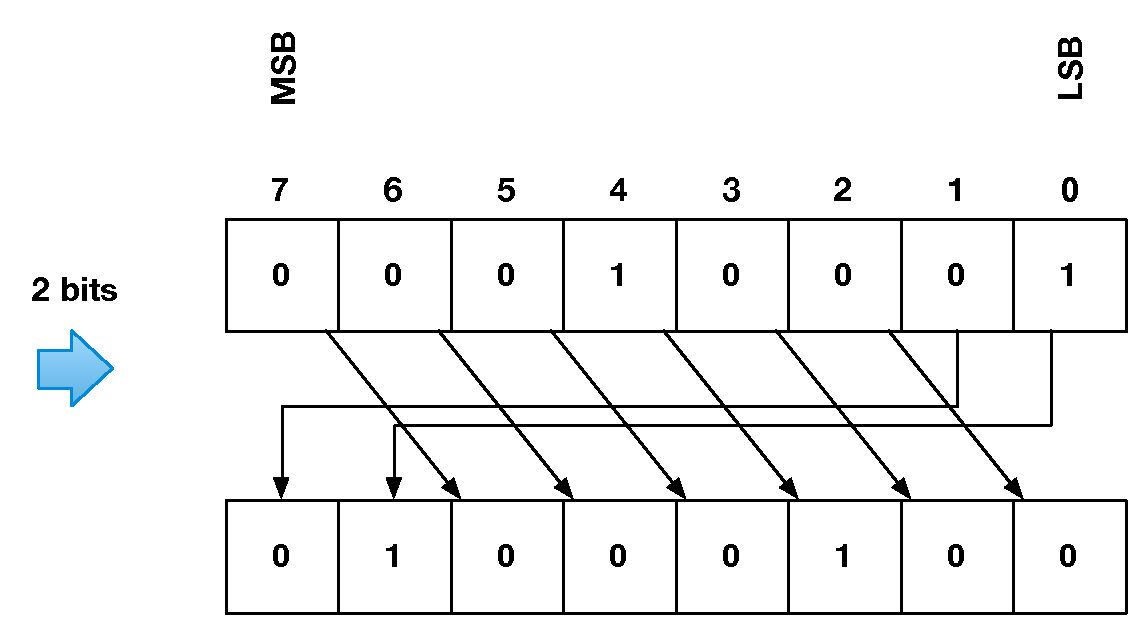
\includegraphics[width=1\textwidth]{./diagrams/r_s_2bits.pdf} \\
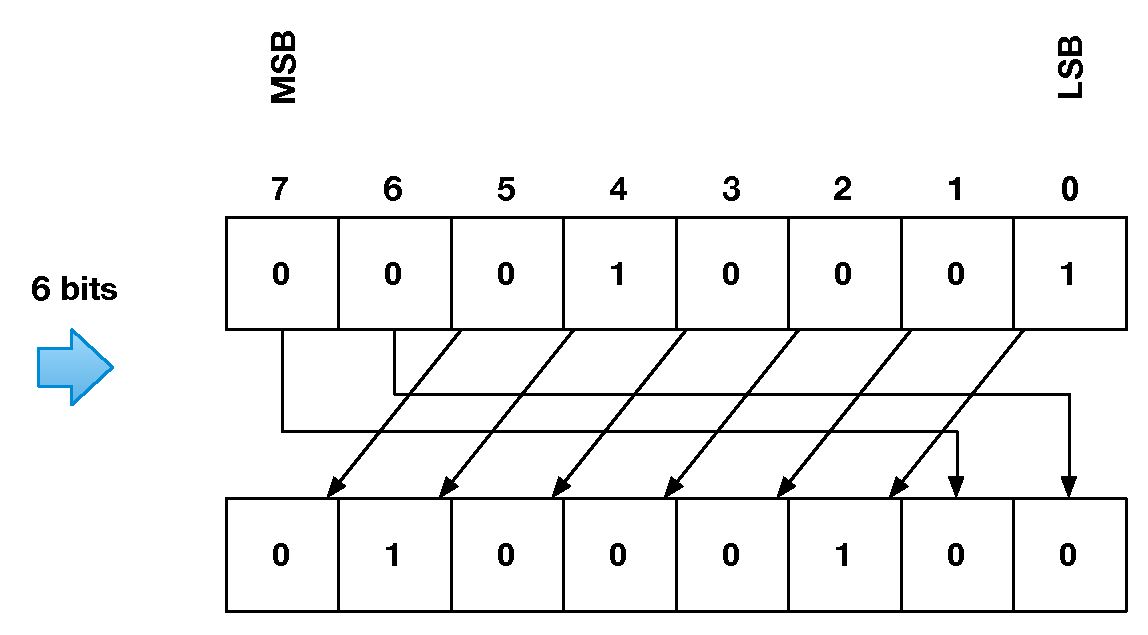
\includegraphics[width=1\textwidth]{./diagrams/r_s_6bits.pdf}
\end{minipage}
}
\subfigure[Different Blocks Shifted Different Bits]{
\begin{minipage}[b]{0.45\textwidth}
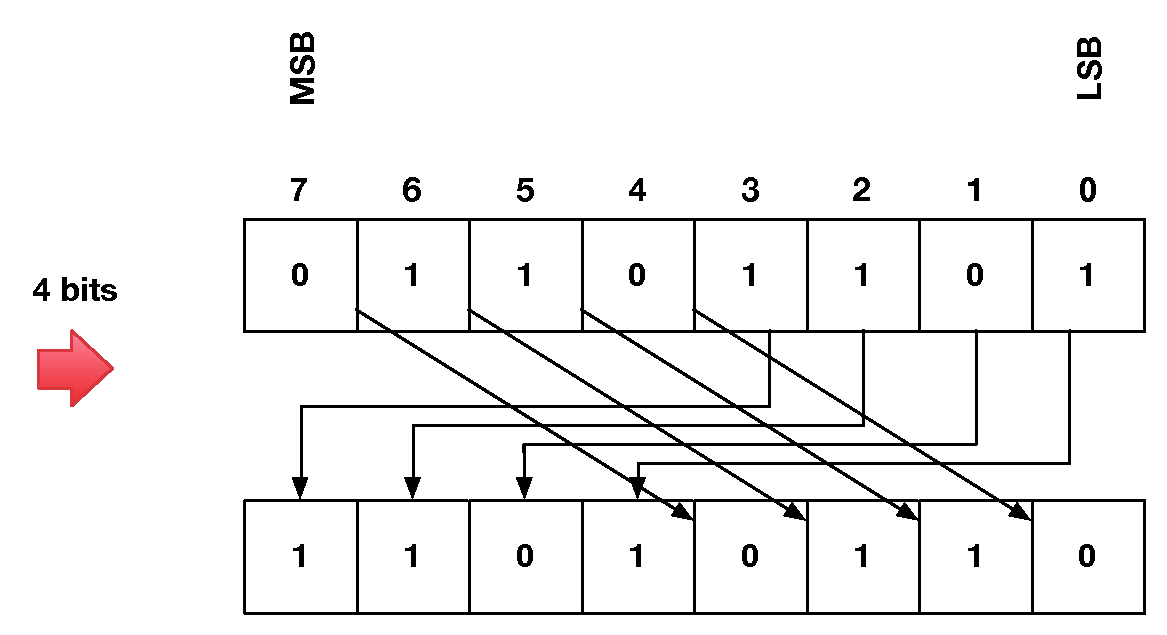
\includegraphics[width=1\textwidth]{./diagrams/r_d_4bits.pdf} \\
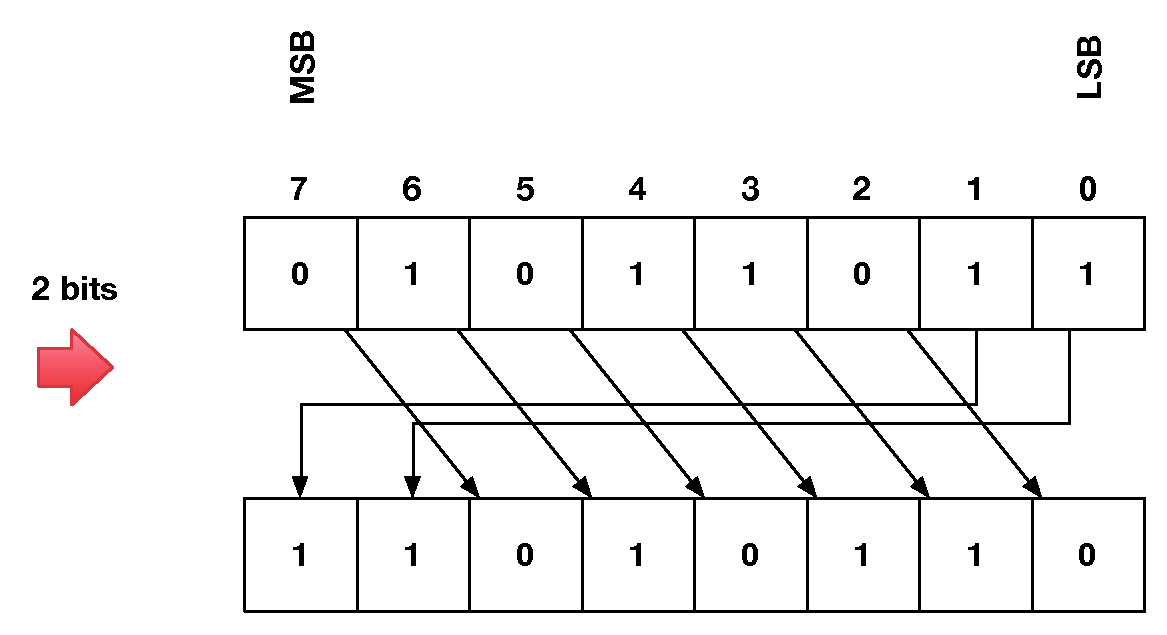
\includegraphics[width=1\textwidth]{./diagrams/r_d_2bits.pdf}
\end{minipage}
}
 \caption{The Examples of Y Block Collision}
 \label{fig: Y-blk-collision}
\end{figure}
Figure $\ref{Y-blk-collision}$ gives the examples of the outputs from shifting
stage that lead tag collision. There are two types of repeated X sets leading to
high probability of tag collision, denoted as sequence-level pattern and
set-level pattern.
\paragraph{The Sequence-level Pattern Collision}
Firstly, we treat blocks as a block sequences, which means in a block sequence, each block has a unique index. The definition of block sequence equality is expressed below:
\begin{defination}
Sequence Equality: Two block sequences X1 and X2 are equal in sequence-level if X$_1$[i] is identical to X$_2$[i] for any i$\in$[1,x].
\end{defination}

Assume the shuffle stage does not work, then the following fact exist:
\begin{itemize}
	\item X1 and X2 are two identical block sequences in sequence-level
\end{itemize}

In block-level rotate shifting stage, a segment from nonce, marked as S, is adopted as the parameter of shifting bits. S is a concatenation of sub-blocks and is denoted as S=(S[1]$\|$S[2]$\ldots$S[x]), where x is the number of blocks in X sequence. The value of S[i] the bits shifted for X[i] block.
For two identical blocks X$_1$[i] and X$_2$[i], the output blocks Y$_1$[i] and Y$_2$[i] are identical if S$_1$[i] is identical to S$_2$[i]. We found that Y$_1$[i] and Y$_2$[i] still have probability to be identical if X$_1$[i] is formed by a repeated short bit segment named pattern. This property is depicted in Proposition 1.1:
\begin{theorem}
Let X$_1$[i] and X$_2$[i] be two identical block and len(X$_1$[i])=N, N=2$^n$. Let S$_1$[i] and S$_2$[i] be two distinct shifting bit parameters for X$_1$[i] and X$_2$[i].
Then Y$_1$[i] and Y$_2$[i] can be identical only when X$_1$[i] is formed by repeating a binary bit segment named pattern and marked as P. The length of P len(P) has the following format:
	P\_L = 2$^p$, p$\in$[0,n-1]
\label{sequence-pattern}
\end{theorem}
Base on Theorem $\ref{sequence-pattern}$, we got the following corollaries:
\begin{corollary}
If a pattern P is not formed by a sub-pattern with shorter length, we call P a distinct pattern with length P\_L. The No. of distinct patterns with length P\_L=2$^p$ is 2$^{2^p}$-2$^{2^{p-1}}$
\label{distinct-pattern}
\end{corollary}
\begin{corollary}
Assume the length of a pattern-forming X block is N=2$^n$, then the No. of all possible distinct patterns is 2$^{N/2}$
\label{pattern-no}
\end{corollary}

From Corollary 1.3 we can see that when the adversary conducts the replay attack on the data concatenated by pattern-formed blocks, the probability that Y block collision is high when shuffle stage does not work. The proof of Theorem $\ref{sequence-pattern}$, Corollary $\ref{distinct-pattern}$ and $\ref{pattern-no}$ is expressed in the appendix. 

\paragraph{The Probability of Tag Collision Under Sequence Pattern Attack}
For two identical X blocks X\_A[i] and X\_B[i], the probability that Y\_A[i]=Y\_B[i] when R\_A[i] and R\_B[i] are randomly generated is marked as  Pr[Y block collision]. 
Pr[Y block collision] is expressed in Theorem $\ref{sequence-prob}$:
\begin{theorem}
Assume for two identical blocks X$_1$[i] and X$_2$[i] the length is N=2$^n$, and the pattern length P$_l$=2$^p$ where p$\in$[0,n-1]. If the pattern contains no internal sub-pattern, then :
\begin{equation}
$$Pr[Y$_1$[i]=Y$_2$[i]] = 1/2$^p$$$
\end{equation}
If the pattern length in X[i] is identical for any i$\in$[1,x] where x is the number of blocks in X sequence, then:
\begin{equation}
$$Pr[Y$_1$[i]=Y$_2$[i]] = (1/2$^p$)$^x$$$
\end{equation}
\label{sequence-prob}
\end{theorem}

\paragraph{The Set-level Pattern Collision}
Secondly we treat blocks as a set allowing the existence of identical elements. We give the definition of block set equality below:
\begin{defination}
Set Equality: Two block sets X1 and X2 are identical in set-level if the following properties are met:
\begin{itemize}
	\item X1 and X2 have same number of elements
	\item The number of elements for each distinct value in X1 is identical to the number in X2
\end{itemize}
\end{defination}

When none of block in a X block sequence is formed by repeated pattern, it is impossible to make two Y sequences with block sequence equality by using two distinct s sequences. This assertion can be proved based on the proof of Proposition 1.1. However, we found that it is possible to form two Y sets with block set equality by using two distinct s sequences. The set-level identical Y sets can lead to tag collision directly. This attack is expressed in Proposition 1.2:
\begin{theorem}
Let X$_1$[i] and X$_2$[j] be two distinct block and len(X$_1$[i])=len(X$_2$[j])=N, N=2$^n$. Let S$_1$[i] and S$_2$[j] be two distinct blocks of shifting bit parameters for X$_1$[i] and X$_2$[j].
Then Y$_1$[i] and Y$_2$[j] can be identical if and only if X$_1$[i] can be formed by rotate shifting X$_2$[j].
\label{set-pattern}
\end{theorem}
Based on Theorem 1.3, we got the following corollary:
\begin{corollary}
For the rotate shifting stage, when the distinct input blocks X$_1$[i] and X$_2$[j] have the property that X$_1$[i] can be formed by rotate shifting X$_2$[j],and the shifting bits parameter S$_1$[i] and S$_2$[j] are distinct, the probability that the output blocks Y$_1$[i] and Y$_2$[j] are identical is Pr[Y$_1$[i]=Y$_2$[j]]=
\end{corollary}
Assume the shuffle stage does not work. When the adversary conducts replay attack on the memory frame whose data part is concatenated by blocks that are formated by shifting a common base block, then each element in X1 sequence can be formed by rotate shifting another element and the probability of forming identical Y sets is high, which will lead to tag collision.

\paragraph{The Probability of Tag Collision Under Set Pattern Attack}
Assume two identical sets X\_A and X\_B satisfy the following properties:
\begin{itemize}
	\item Each element can be formed by rotate shifting any other element in the set
	\item None of the elements is formed by pattern.
\end{itemize}
As each element in the X set can be formed by rotate shifting a base block, we call such X set Same Base Block(SBB) X sets, short for SBB X sets. If none of the element is formed by a pattern ,we call such X set SBB only sets.

From Corollary 1.3 we know that for a block that is N bits long, the No. of possible values that is formed by a pattern is 2$^{N/2}$, which also means the No. of distinct values that is not formed by a pattern is 2$^{N/2}$. Assume D\_A and D\_B are randomly generated, the probability of generating SBB only D set is expressed:
\begin{defination}
Pr[ SBB only D(X)] =
\begin{equation}
2^{n/2} * N^{M-1} / (2^N)^M
\end{equation}
\end{defination} 

Using SBB only X\_A and X\_B, the probability of CIE of Y\_A and Y\_B is marked as Pr[CIE Y Sets] and expressed as the following way:
\begin{defination}
Pr[CIE Y Sets] = $$\prod_{i=1,j=1}^M Pr[Y\_A[i] = Y\_B[j]]$$ where M is the No. of elements in a set, i,j$\in$[1,M] and i$\neq$j
\end{defination} 

For two randomly generated R\_A and R\_B, the probability that Y\_A and Y\_B are CIE when X\_A and X\_B are SBB only is expressed in the following theorem:
\begin{theorem}
Assume X\_A and X\_B are SBB only, R\_A and R\_B are randomly generated,then:

Pr[CIE Y Sets]:
\begin{displaymath}
(\sum_{K=1}^{min(N,M)} \binom{N}{K} * (M!/v1!v2!v3! \cdots vk!) ^ 2 )/(N^M)^2
\end{displaymath}
\label{set-prob}
\end{theorem}

\subsubsection{The Vulnerable Inputs Set of CETD-MAC Under Replay Attack}
As summarized before, the shuffle stage is vulnerable to inputs that is unbalanced in the percentage of 0s and 1s. After splitting a input to blocks, shuffle stage cannot effectively change the bit distribution of input blocks and the output of shuffle stage, X blocks, have big probability to be identical to the input.
On the other hand, shifting stage if vulnurable to the input formed with a type of patterns. The patterns can exist in sequence level or set level. The pattern in the input of shifting stage have good chance to induce identical Y sets and directly produce tag collisions. 
We can see that if the input chosen by the adversary for replay attacks is the in the intersection of vulunrable inputs of shuffle and shifting stage, then there is good chance to form identical Y sets even if the nonce is generated from secure block cipher encryption. 

\paragraph{The Case of Input Trigging Two Pattern Attacks}
If the blocks in X set is formed by rotate shifting a base block and this base block is formed by a pattern, then such X set pair X\_A and X\_B can result either IIE or CIE Y set pairs.

Assume the R\_A and R\_B are randomly generated, the probability that Y\_A and Y\_B are SLE is expressed in the following theorem:
\begin{theorem}
Assume X\_A and X\_B are both SBB and IPL, R\_A and R\_B are randomly generated,then:

Pr[SLE Y Sets]=
\begin{displaymath}
(\sum_{K=1}^{min(N,M)} \binom{N}{K} * (M!/v1!v2!v3! \cdots vk!) ^ 2 )/(N^M)^2
\end{displaymath}
\end{theorem}
The proof of theorems is expressed in the appendix.

\paragraph{The Behaviour of X Blocks from Shuffling Stage}
\begin{figure}
\centering
\subfigure[Only Single Block Equality]{
 \label{fig:y_single_e} %% label for first subfigure
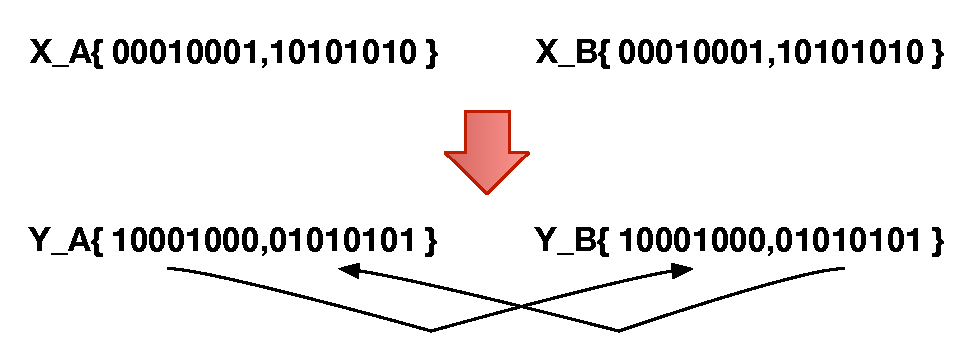
\includegraphics[width=.5\textwidth]{./diagrams/y_single_equality.pdf}
}
%\hspace{1in}
\subfigure[Only Set Level Equality]{
\label{fig:y_set_e} %% label for second subfigure
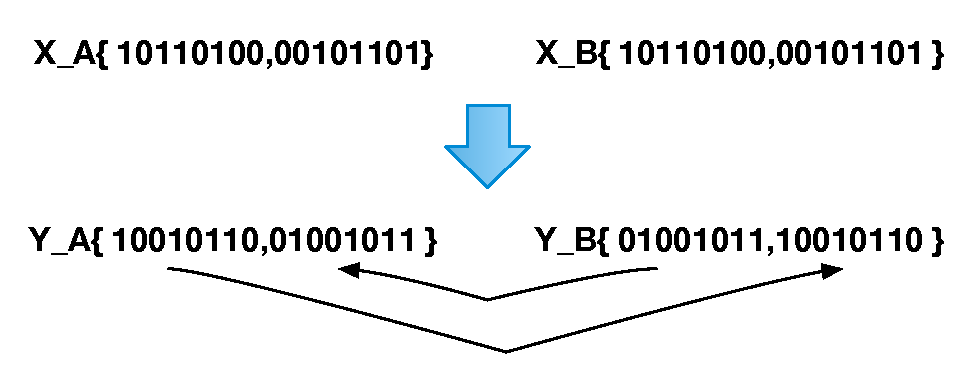
\includegraphics[width=.5\textwidth]{./diagrams/y_set_equality.pdf}
}
\caption{X Set Pairs with Only One Type of Y Equality}
 \label{fig:y_e_single} %% label for entire figure
\end{figure}

\begin{figure}
\centering
\subfigure[Single Block Equality Case]{
 \label{fig:y_both_single} %% label for first subfigure
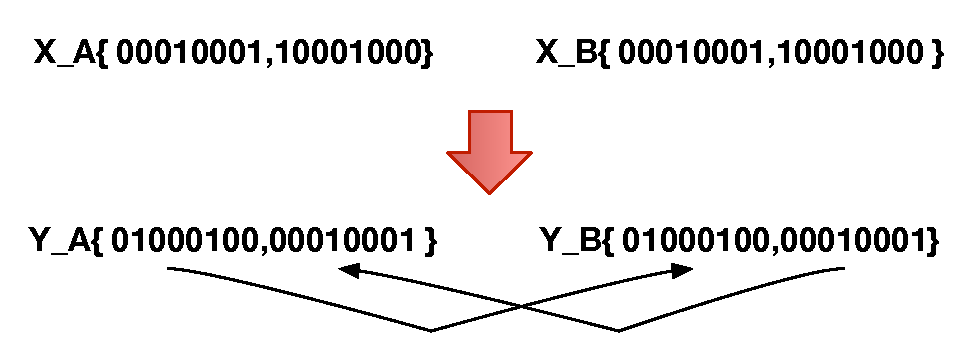
\includegraphics[width=.5\textwidth]{./diagrams/y_both_single.pdf}
}
%\hspace{1in}
\subfigure[Set Level Equality Case]{
\label{fig:y_both_set} %% label for second subfigure
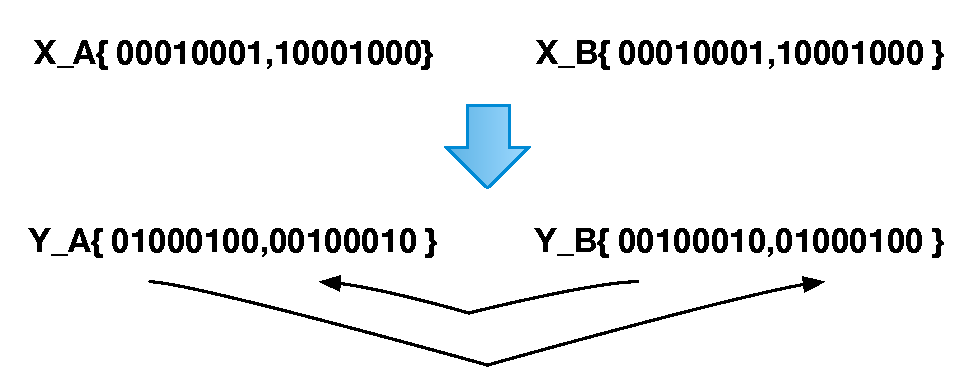
\includegraphics[width=.5\textwidth]{./diagrams/y_both_set.pdf}
}
\caption{A X Set Pair with Two Types of Y Equality}
 \label{fig:y_both} %% label for entire figure
\end{figure}
In each round of Shuffle stage, two blocks from the output of previous round of shuffle are randomly selected then operate bit segments swapping, which will effect the distribution of bits in the two blocks. After the shuffle stage, the output, X blocks, can be classified to four categories:
\begin{enumerate}
	\item Formed by repeated patterns
	\item Formed by rotate shifting another block in this category
	\item Contains the properties from categories 1 and 2
	\item No properties from categories 1 or 2
\end{enumerate}
Assume the block cipher used in nonce generation performances like PRF, the number of blocks in each category is effected by the input message M and the rounds of shuffle stage.  

\subsection{Security Enhanced CETD-MAC}
In this section we provide an modification of original CETD-MAC. Our approach does not require additional component or information to the original CETD-MAC. We then prove that the optimized CETD-MAC can fix the weakness and protect input message from replay attack.
\paragraph{Inspiration}
As depicted above, if a input message is consisted of blocks formed with a type of pattern and the proportion of 0s and 1s in the message is extremely unbalanced, the message cannot be effectively randomized by neither the shuffle stage nor the shifting stage. That means the message has high probability to induce identical Y sets or Y sequences under replay attack. The identical Y sets or Y sequences will directly induce tag collision then succeed the replay attack. 
\paragraph{Question}
Using only shuffle and shift with random nonce, is it possible to ensure the range of tag to 2$^n$? If not, why?

\section{Experiments and Results}
\appendix
\section{Proof of Assertions}
\subsection{Proof of Theorem 1.1}
This part proves that if two identical block X\_A[i]  and X\_B[i] are shifted different bits and the result blocks remain identical, X\_A[i] is formed by pattern. The pattern length and $\delta$=$\mid$R\_A[i]-R\_B[i] $\mid$ has such correlation:
\begin{itemize}
	\item If $\Delta$ = P\_L then Y\_A[i] = Y\_B[i] where P\_L the length of pattern
\end{itemize}
Assume the length of X\_A[i] is N bits, where N= 2$^n$. When X\_A[i] is formed by a pattern whose length is P\_L = 2$^p$ bits, then the domain of Y\_A[i] has P\_L distinct values. There are N/P\_L distinct R\_A[i] values that shift X\_A[i] to a Y\_A[i].  

\subsection{Proof of Theorem 1.3}
If two distinct X blocks result two identical Y block. Assume the shift bits parameter blocks are R\_A[i] and R\_B[i]. Then X\_A[i] can be formed by rotate shifting Y\_A[i] for (N-R\_A[i]) mod N bits. X\_B[i] can be formed for (N-R\_B[i]) mod N bits.
X\_B[i] can be formed by rotate shifting X\_A[i] for (R\_A[i] + N-R\_B[i]) mod N bits. Theorem 1.2 proved.

\section{Computation Procedure of Probabilities}
\subsection{Proof of Theorem 1.2}
For identical each block pair X\_A[i] and X\_B[i], the No. of combination of R\_A[i] and R\_B[i] = N*N, where N is the length a X block. 
If X\_A[i] is formed by pattern, then Y\_A[i]=Y\_B[i] if $\mid$R\_A[i]-R\_B[i]$\mid$ = P\_L * K, where P\_L is the pattern length and K is a positive integer. 
Then for two random R\_A[i] and R\_B[i], Pr[Y\_A[i]=Y\_B[i] $\mid$ X\_A[i] = X\_B[i] \& pattern = P\_L](shoft for Pr[Y\_A[i] = Y\_B[i]]) can be expressed in the following way:
\begin{itemize}
	\item Pr[Y\_A[i]=Y\_B[i]] = N * (N/P\_L)/(N*N) = 1/P\_L
\end{itemize} 

\subsection{Proof of Theorem 1.4}
From Theorem 1.1 we can see that if a X block is formed by a pattern, then the No. of distinct values in the range of Y block is P\_L. While the domain of a R block has N distinct values, then for a block X, there are N/P\_L distinct R values that lead to a Y value.

If a X block is not formed by a pattern, then for each distinct R value, there is a distinct Y value. That means for a given X set that none of the blocks is formed by a pattern, each R set will lead to a distinct Y set. The map between R set and Y set is bijection.

When each R block is randomly generated, the possible combination of R sets is N$^M$. That means for a given X set, the No. of possible Y set is N$^M$.

Assume X\_A and X\_B are IIE and each block can be formed by rotate shifting another block in the set. On the other hand, none of blocks is formed by a pattern. Then the sub-group of blocks in X\_A and X\_B can form CIE with specific R\_A and R\_B set. 

Assume set Y\_A and Y\_B are SLE, then Y\_B is a permutation of Y\_A. This concept can be modeled in the following way:
\begin{itemize}
	\item Assume the M elements in Y\_A contain K distinct values. The No. of the elements that have each value are marked as v1,v2...vk.
	\item IF the elements in Y\_B are a permutation of the elements in Y\_A, then Y\_A and Y\_B are SLE.
\end{itemize}

Based on the basic concept in Combinatorics, the No. of a permutation of Y\_A that contains K distinct value can be expressed in the following equation:
\begin{defination}
No. of Permutation with K distinct Values:
\begin{displaymath}
\binom{M}{v1} * \binom{M-v1}{v2} * \binom{M-v1-v2}{v3} \cdots * \binom{vk}{vk} = M!/v1!v2!v3! \cdots vk!
\end{displaymath}
\end{defination}
As any one of the elements in X set can be formed by rotate shifting another element, then the No. of distinct values of M elements, K, various from 1 to M. If Y\_A has K distinct values, the No. of possible combination of these K elements in Y\_A can be expressed as Com\_Y\_A:
\begin{defination}
Com\_Y\_A:
\begin{displaymath}
M!/v1!v2!v3! \cdots vk!
\end{displaymath} 
\end{defination} 

For each case of Y\_A in Com\_Y\_A, the No. of Y\_B to form SLE is also Com\_Y\_A. Then if Y\_A has K distinct values, Pr[CIE Y sets] can be expressed as:
\begin{defination}
Pr[CIE Y Sets]:
\begin{displaymath}
 \binom{N}{K} * (M!/v1!v2!v3! \cdots vk!) ^ 2 /(N^M)^2
\end{displaymath}
\end{defination}
If R\_A and R\_B are randomly generated, then the value of K various from 1 to M. We do th sum to get the expression in Theorem 1.4
\begin{defination}
Pr[CIE Y Sets]:
\begin{displaymath}
(\sum_{K=1}^{min(N,M)} \binom{N}{K} * (M!/v1!v2!v3! \cdots vk!) ^ 2 )/(N^M)^2
\end{displaymath}
\end{defination}

\subsection{Proof of Theorem 1.5}
If the element contains both the properties of CIE and IIE, then the following properties:
\begin{itemize}
	\item For two distinct sets R\_A and R\_B, Y\_A and Y\_B can be IIE
	\item For each value of a Y block, there are N/P\_L distinct R block that can shift X to this Y. That means for a distinct Y set, the No. of R sets is not one.
	\item For two distinct sets R\_A and R\_B, Y\_A and Y\_B can be CIE
\end{itemize}
Base on the Theorem 1.1, if the X block is formed by pattern, then the No. of values in the range of Y is P\_L, base on theorem 1.4, the Pr[SLE Y sets] can be expressed as:
\begin{defination}
Pr[SLE Y Sets:]:
\begin{displaymath}
\binom{P\_L}{K} * (M!/v1!v2!v3! \cdots vk!) ^ 2 )/(P\_L^M)^2
\end{displaymath}
\end{defination}

If R\_A and R\_B are randomly generated, then the value of K various from 1 to M. We do th sum to get the expression in Theorem 1.5
\begin{defination}
Pr[SLE Y Sets]:
\begin{displaymath}
(\sum_{K=1}^{min(P\_L,M)} \binom{P\_L}{K} * (M!/v1!v2!v3! \cdots vk!) ^ 2 )/(P\_L^M)^2
\end{displaymath}
\end{defination}



\end{document}
